Di seguito viene riportato il diagramma ER completo dell'applicazione. Il diagramma è stato creato con l'intenzione di essere una guida per la creazione dei modelli, quindi punta ad essere un riflesso di quanto è stato e verrà implementato, invece che una rappresentazione dettagliata della struttura del database. Questo implica che alcuni dettagli non sono esplicitati nel diagramma, perché considerati superflui (perché implementati dal framework) o già presenti nel sistema.

\noindent Sono state adottate le seguenti convenzioni:
\begin{itemize}
	\item tutte le entità che possiedono l'attributo \verb|creator_id| hanno implicitamente una relazione del tipo (1, N) con l'entità \verb|users|. La relazione non è stata rappresentata perché avrebbe aumentato notevolmente la complessità del diagramma, riducendone la leggibilità, al netto di una semplificazione ritenuta sufficientemente intuitiva;
	\item la colonna sinistra delle tabelle indica eventuali proprietà particolari degli attributi:
	\begin{itemize}
		\item N: l'attributo può assumere il valore \verb|NULL|. Di conseguenza si assume che tutti gli attributi che non possiedono questa proprietà vengono considerati \verb|NOT NULL|;
		\item U: l'attributo possiede un indice di unicità, all'interno dell'entità, cioè viene considerato \verb|unique|;
		\item FK: indica gli attributi che sono chiavi esterne (\emph{foreign key}) di altre entità. Non viene specificata l'entità a cui si riferiscono, perché inferita dal nome dell'attributo, come da convenzioni di Rails. Ad eccezione di alcuni casi, comunque ritenuti intuitivi, tutte le chiavi esterne si chiamano \texttt{\emph{entity}\_id}.
	\end{itemize}
	\item la colonna destra delle tabelle indica il tipo dell'attributo utilizzato nella migrazione. L'unica eccezione è il tipo fittizio \verb|BLOB|, che indica che quell'attributo è in realtà un attachment, dichiarato a modello.
\end{itemize}

\begin{figure}[b]
	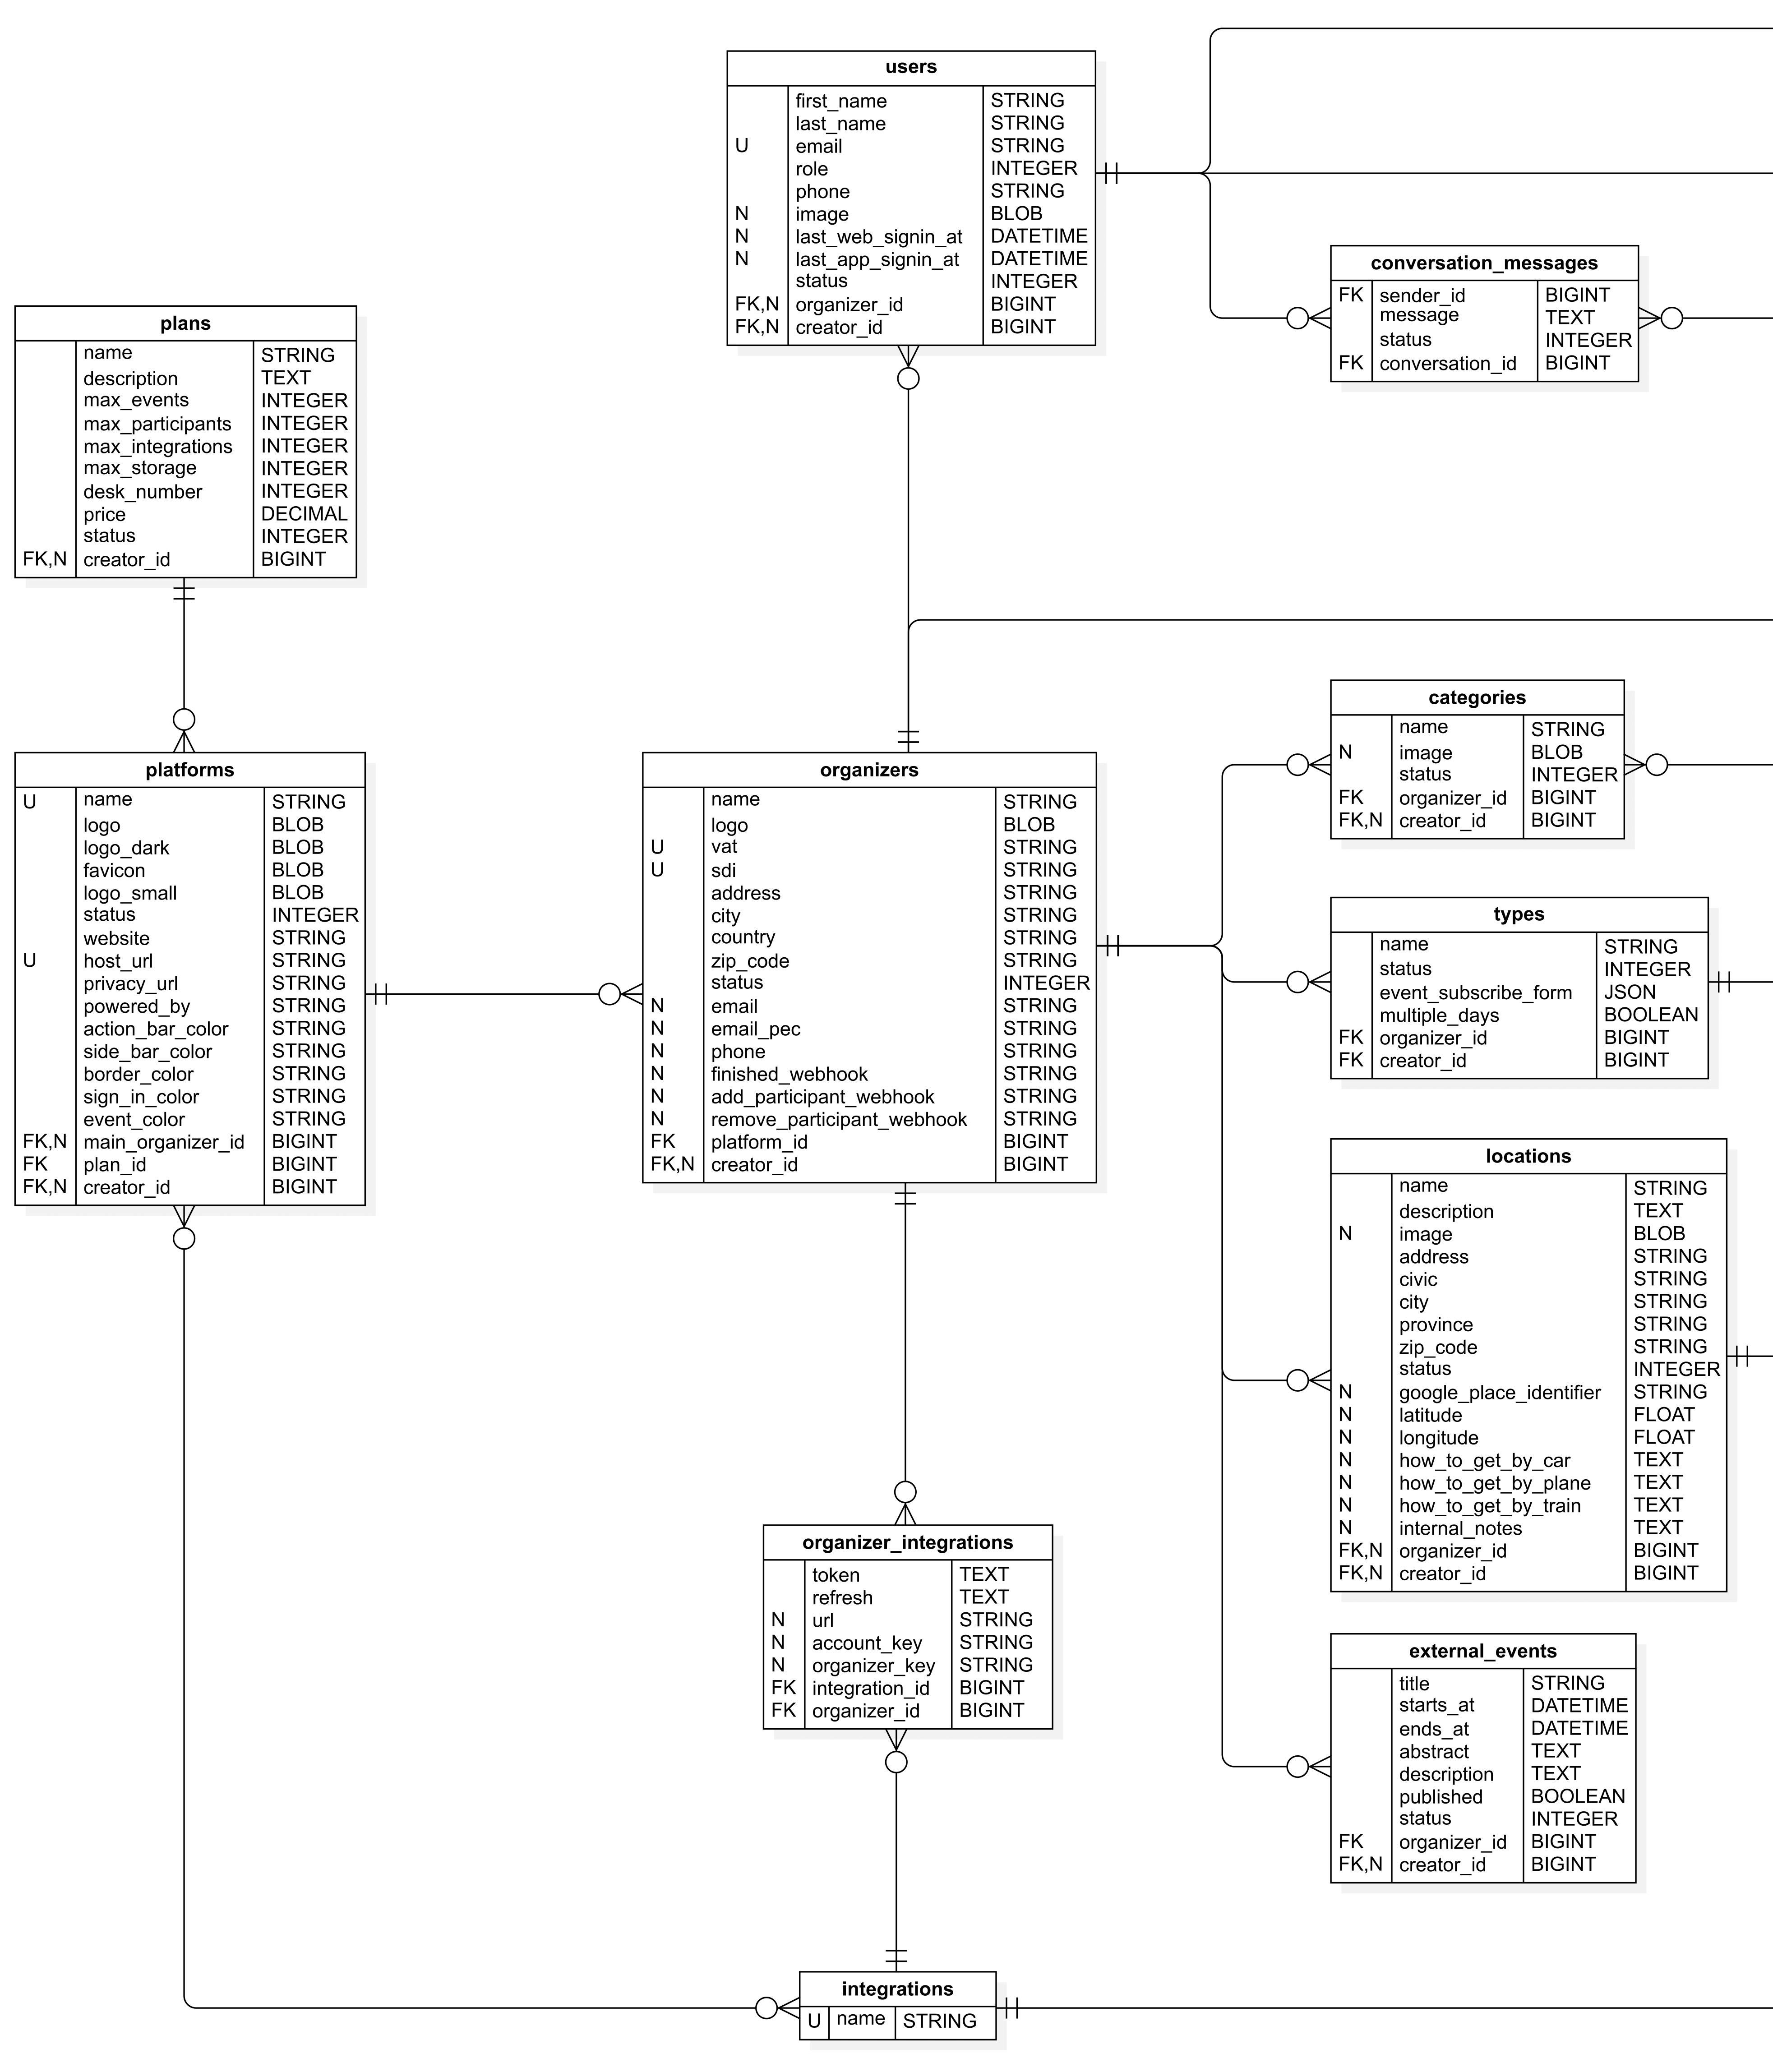
\includegraphics[width = \textwidth]{db/ER-west}
	\caption{Sezione sinistra del dettaglio del diagramma ER}
	\label{fig:er-west}
\end{figure}

\begin{figure}[b]
	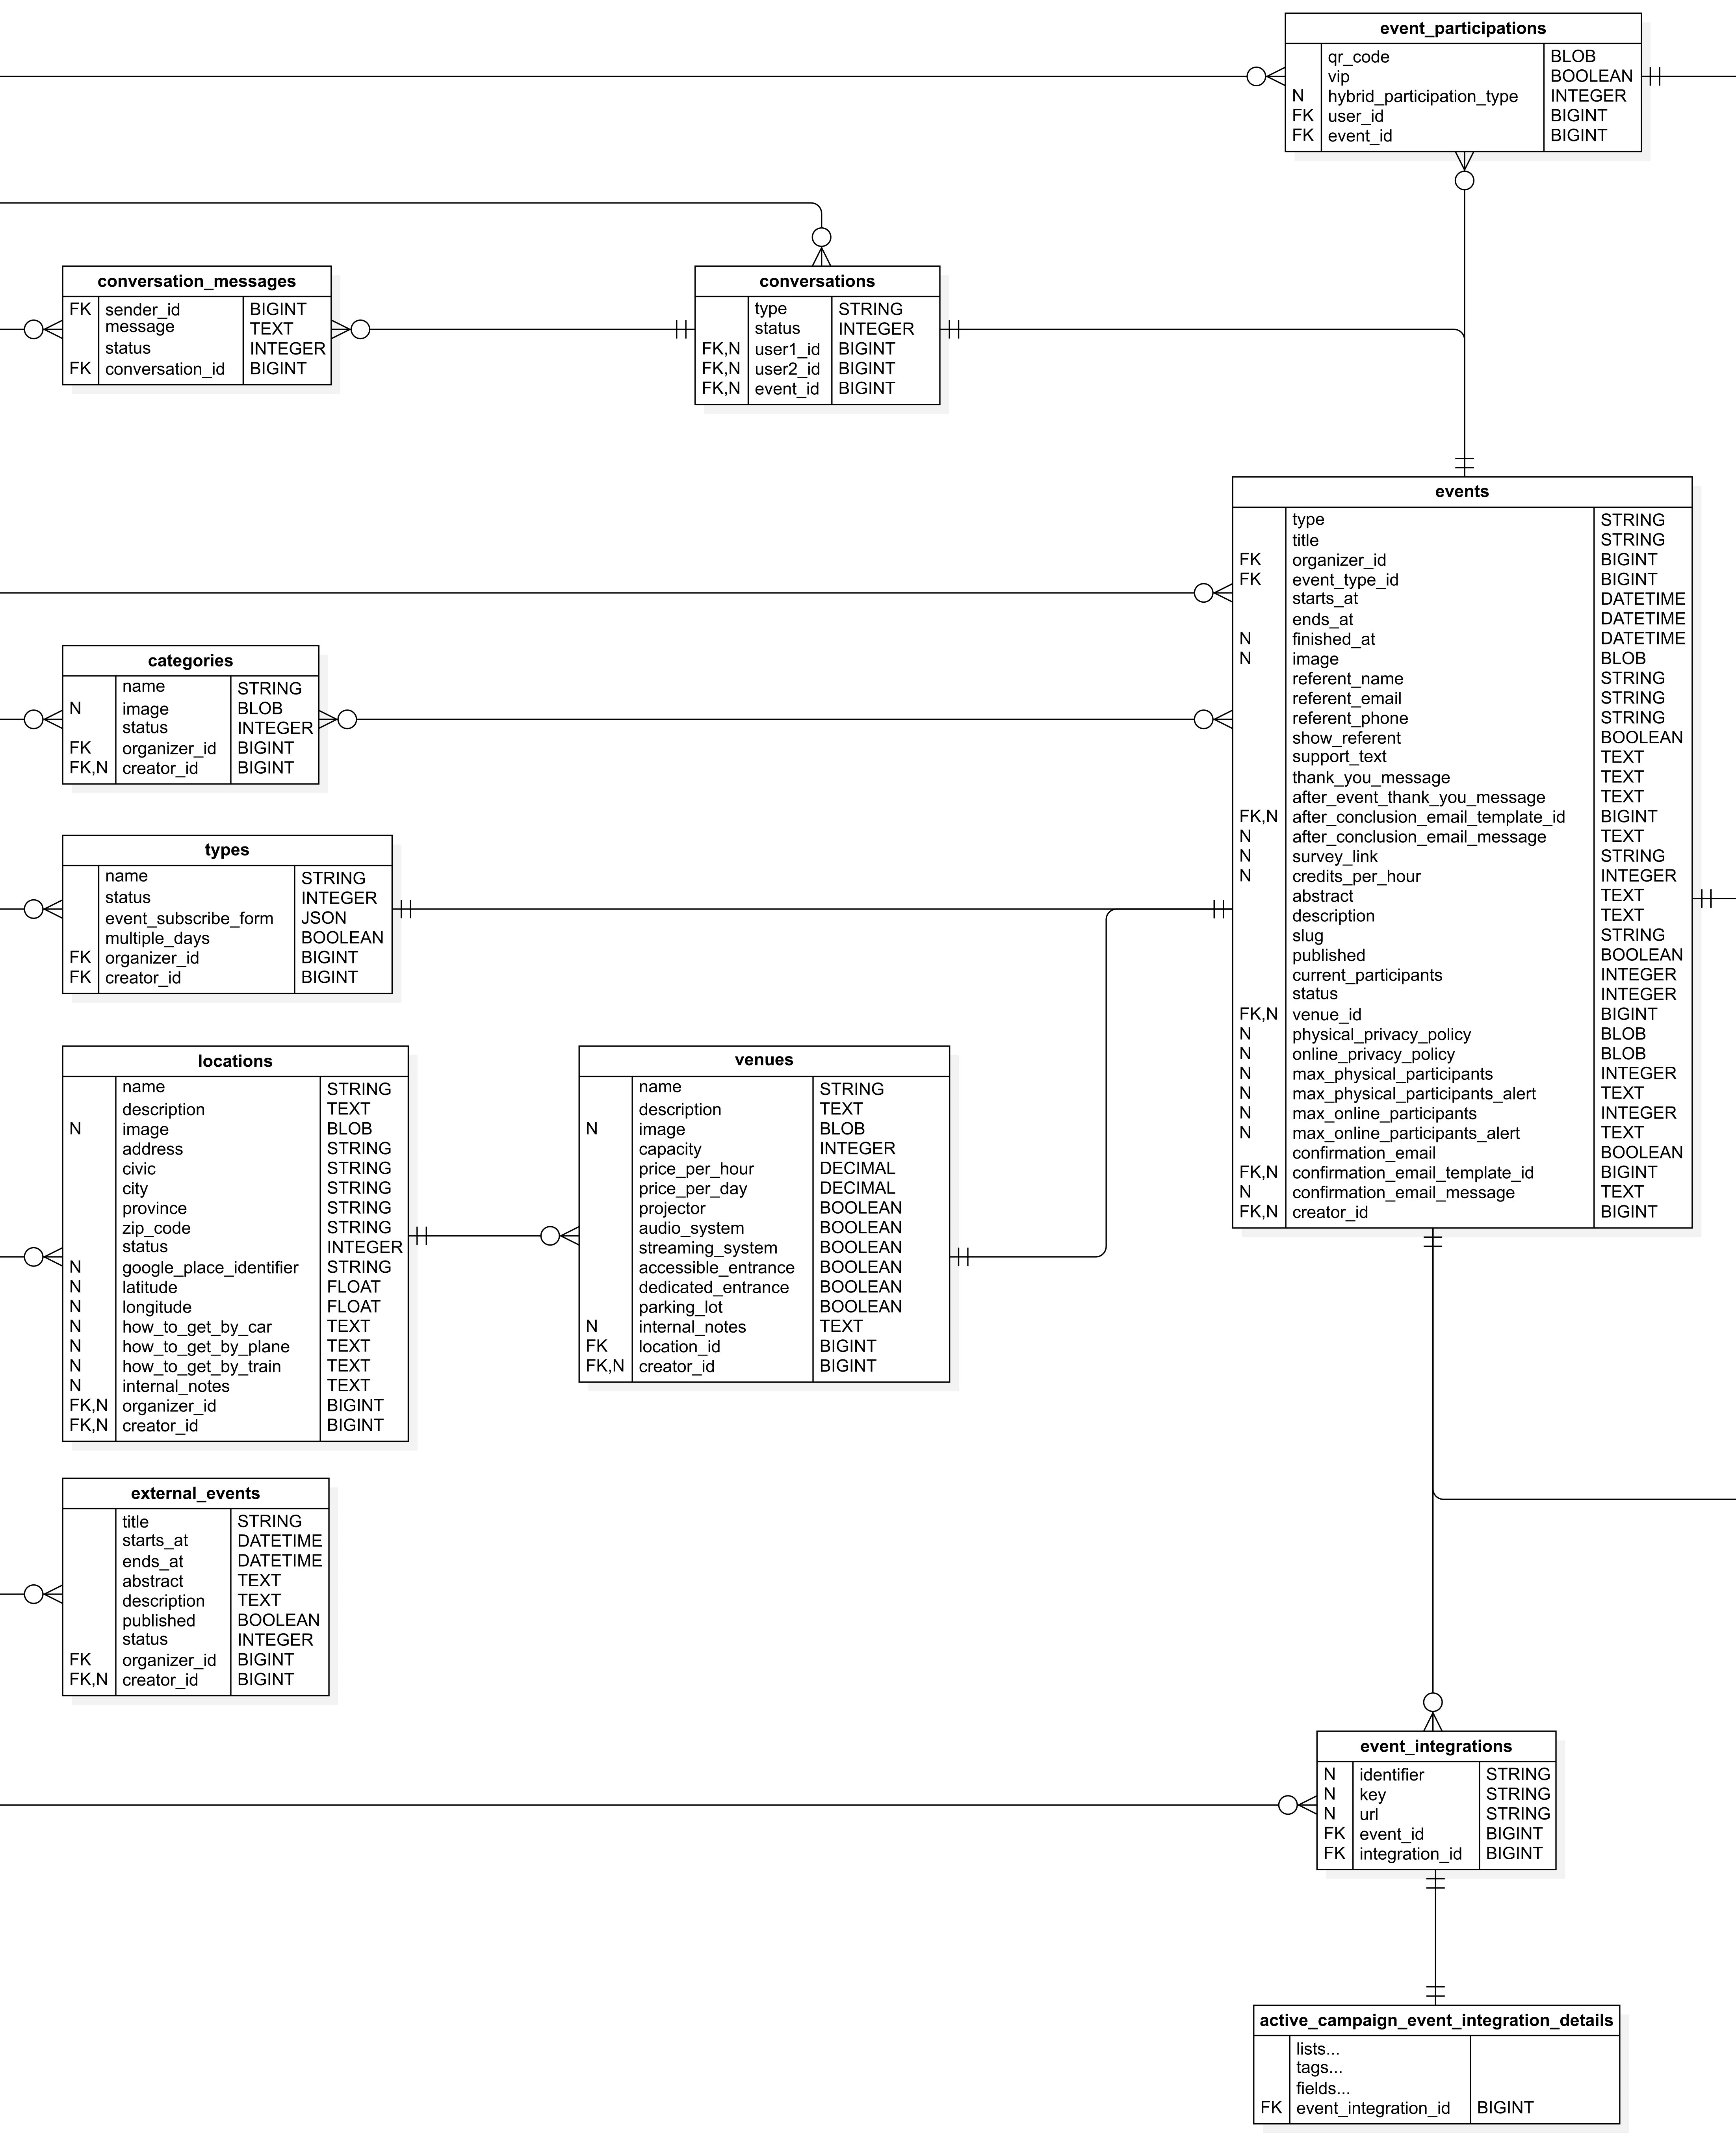
\includegraphics[width = \textwidth]{db/ER-center}
	\caption{Sezione centrale del dettaglio del diagramma ER}
	\label{fig:er-center}
\end{figure}

\begin{figure}[b]
	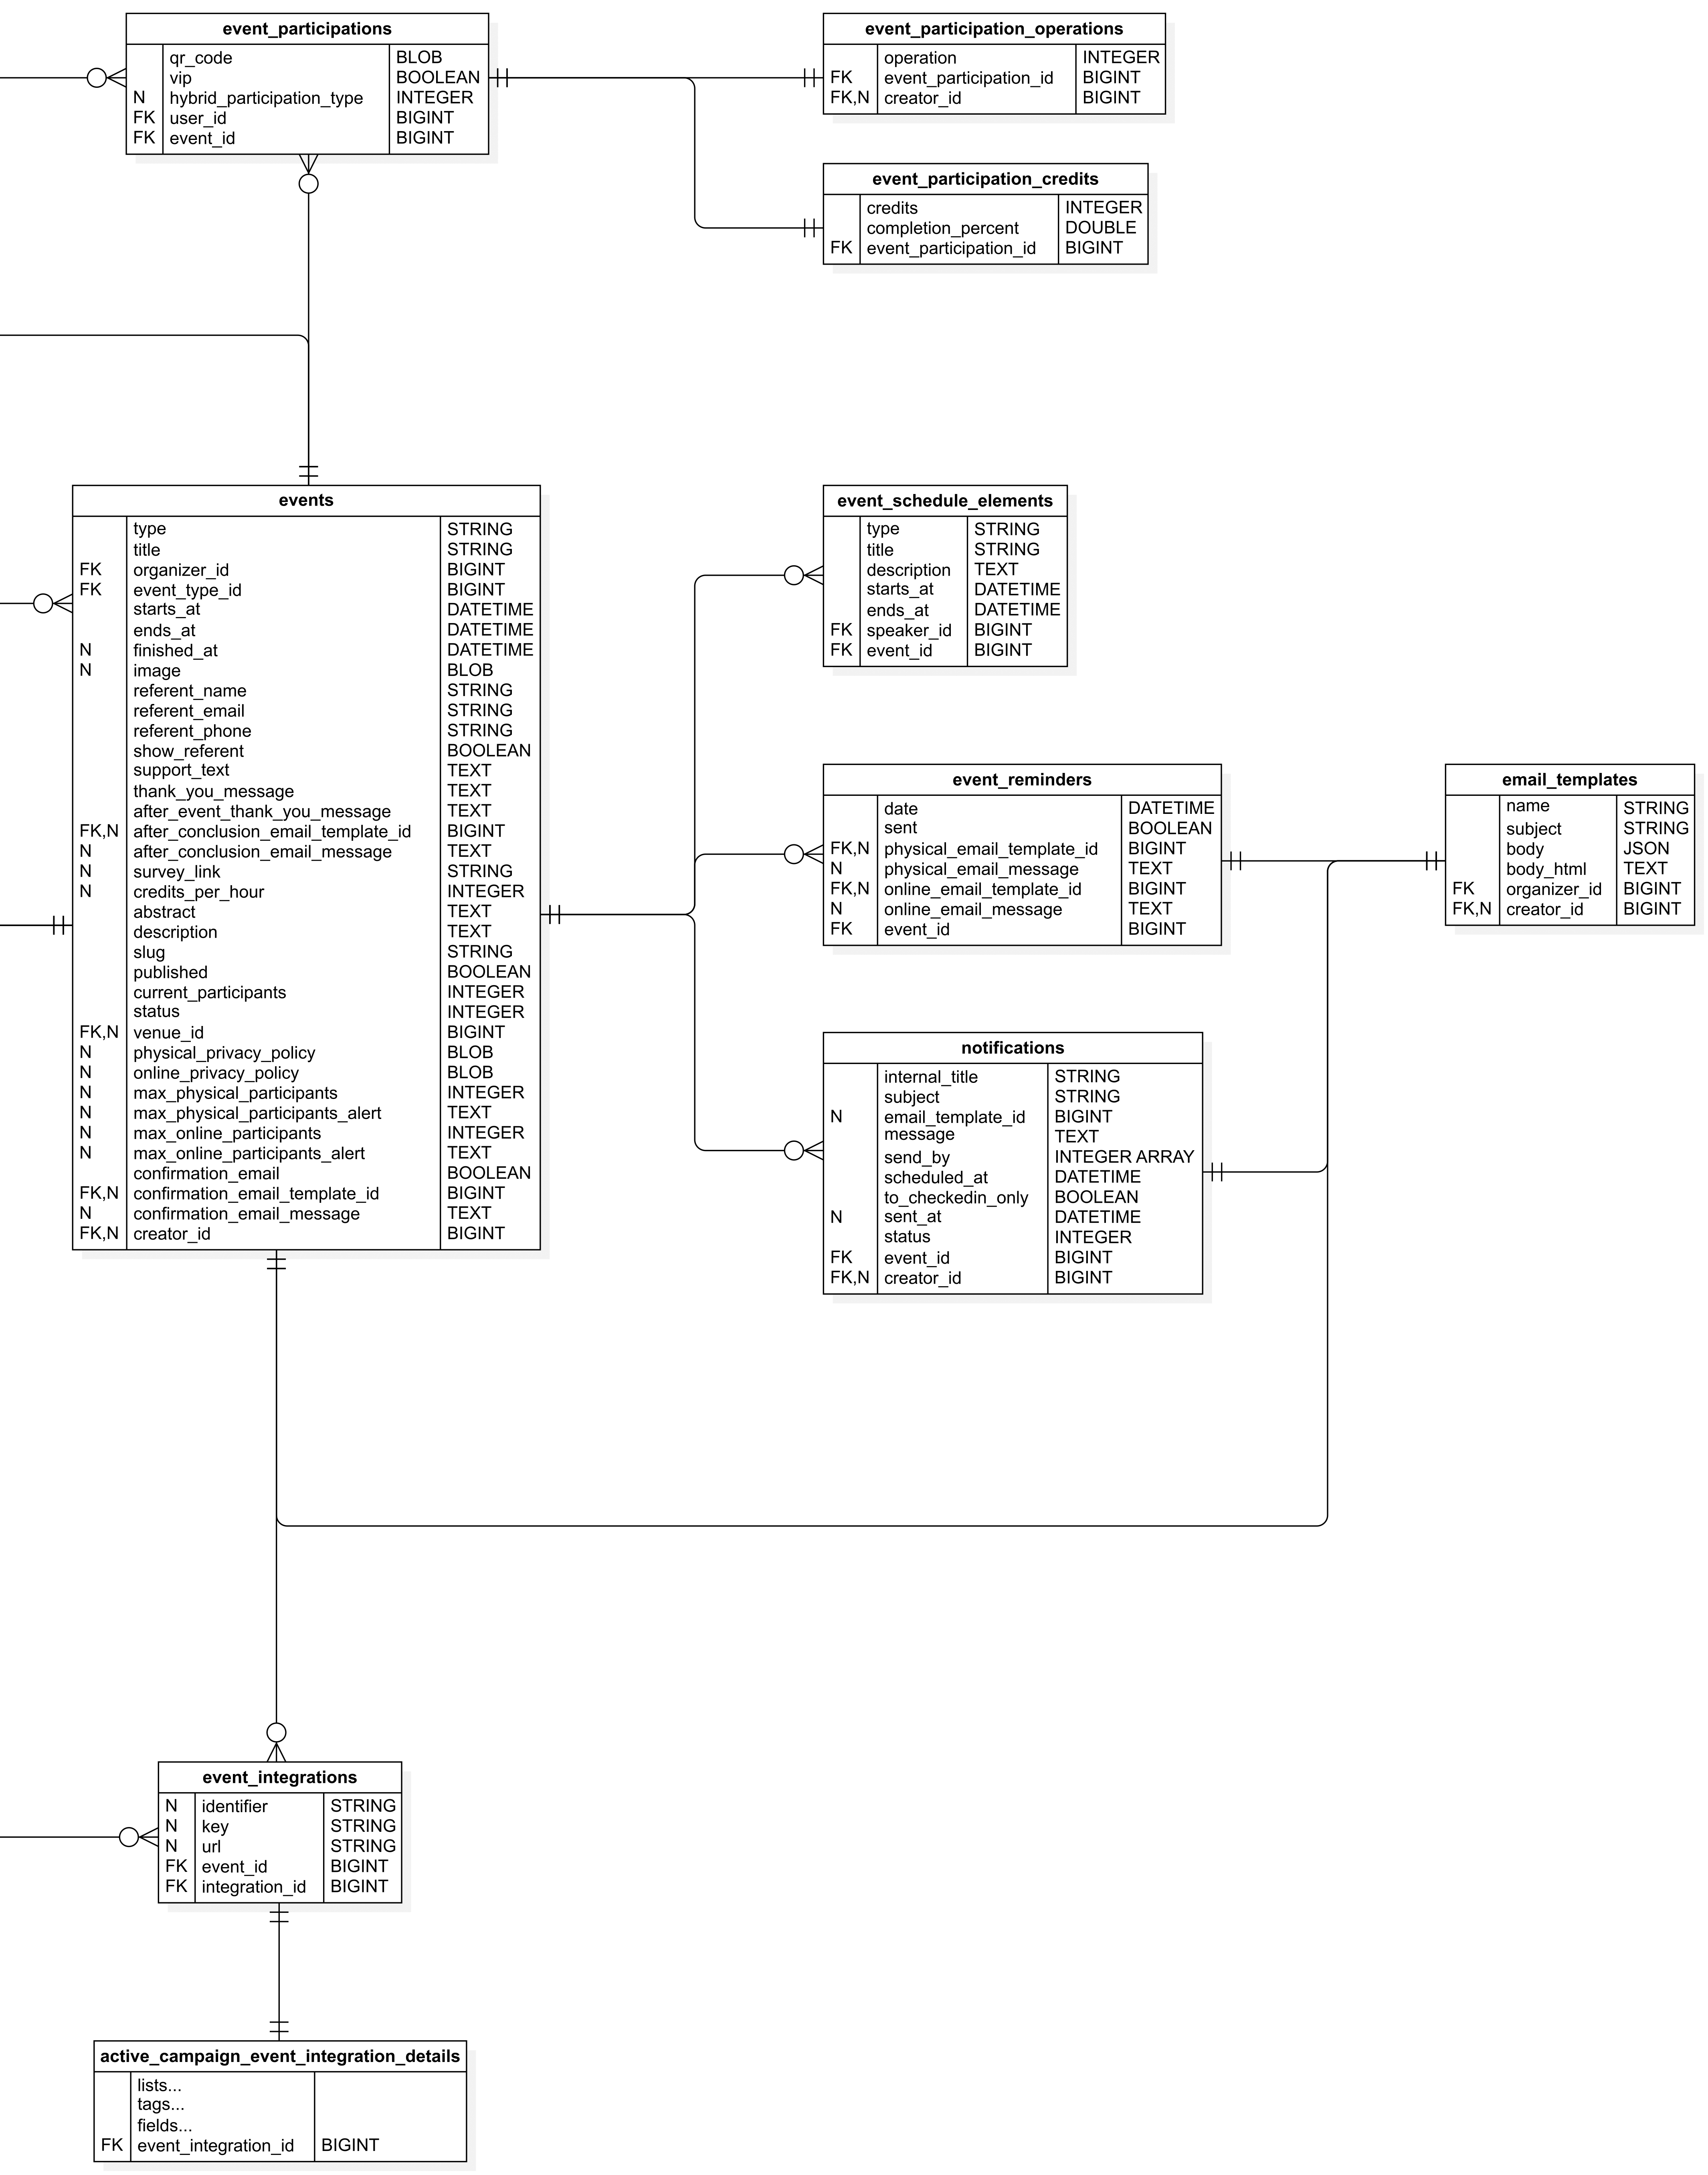
\includegraphics[width = \textwidth]{db/ER-east}
	\caption{Sezione destra del dettaglio del diagramma ER}
	\label{fig:er-east}
\end{figure}
